\qrchapter{https://forgottenpillar.com/rsc/pl-fp-chapter1}{Fundament naszej wiary}

\egw{\textbf{Pan tchnie nową, życiodajną siłę w swoje dzieło}, gdy ludzcy przedstawiciele będą posłuszni rozkazowi, by iść naprzód i głosić prawdę. \textbf{Ten, który oświadczył, że Jego prawda będzie świecić na wieki, będzie głosił tę prawdę przez wiernych posłańców, którzy sprawią, że trąba wyda wyraźny dźwięk}. \textbf{Prawda będzie krytykowana, wyśmiewana i wyszydzana; ale im \underline{dokładniej} będzie badana i poddawana próbie, tym \underline{jaśniej będzie świecić}}}[SpTB02 51.1; 1904][https://egwwritings.org/read?panels=p417.260]

\egwnogap{\textbf{Jako lud mamy \underline{stać niewzruszenie na platformie wiecznej prawdy}, która przetrwała próby i doświadczenia. Mamy \underline{trzymać się pewnych filarów naszej wiary}. \underline{Zasady prawdy}, które Bóg nam objawił, \underline{są naszym jedynym prawdziwym fundamentem}. To one uczyniły nas tym, czym jesteśmy. Upływ czasu nie zmniejszył ich wartości. \underline{Nieustannym wysiłkiem wroga jest usunięcie tych prawd z ich miejsca} i zastąpienie ich \underline{fałszywymi teoriami}. \underline{Wprowadzi on} wszystko, co tylko może, aby zrealizować swoje zwodnicze plany. Lecz Pan wzbudzi ludzi o bystrym umyśle, którzy nadadzą tym prawdom właściwe miejsce w Bożym planie}}[SpTB02 51.2; 1904][https://egwwritings.org/read?panels=p417.261]

\egwnogap{\textbf{Zostałam pouczona przez niebiańskiego posłańca, że część rozumowania w książce «The Living Temple» jest niepoprawna i że \underline{to rozumowanie sprowadziłoby na manowce} umysły tych, którzy nie są całkowicie utwierdzeni w \underline{fundamentalnych zasadach} teraźniejszej prawdy. Wprowadza to, co jest niczym innym jak spekulacją w \underline{odniesieniu do osobowości Boga i tego, gdzie jest Jego obecność}}. Nikt na tej ziemi nie ma prawa spekulować na ten temat. \textbf{Im więcej fantazyjnych teorii staje się przedmiotem dyskusji, tym mniej ludzie będą wiedzieć o Bogu i prawdzie, która uświęca duszę}}[SpTB02 51.3; 1904][https://egwwritings.org/read?panels=p417.262]

\egwnogap{Jeden po drugim przychodzą do mnie z prośbą \textbf{o wyjaśnienie stanowisk zajętych w «The Living Temple»}. Odpowiadam: «\textbf{Są one niewytłumaczalne}». \textbf{Wyrażone tam poglądy nie dają prawdziwego poznania Boga}. W całej książce znajdują się fragmenty Pisma Świętego. Te fragmenty Pisma są przedstawione w taki sposób, że błąd wydaje się być prawdą. \textbf{Błędne teorie są przedstawione w tak ujmujący sposób, że jeśli nie zachowa się ostrożności, wielu zostanie wprowadzonych w błąd}}[SpTB02 52.1; 1904][https://egwwritings.org/read?panels=p417.265]

\egwnogap{\textbf{Nie potrzebujemy mistycyzmu, który jest w tej książce}. Ci, którzy przyjmują te sofizmaty, wkrótce znajdą się w pozycji, gdzie wróg będzie mógł z nimi rozmawiać i odwieść ich od Boga. Zostało mi przedstawione, że autor tej książki jest na fałszywej ścieżce. \textbf{Stracił z oczu charakterystyczne prawdy \underline{na ten czas}}. Nie wie, dokąd prowadzą jego kroki. \textbf{\underline{Ścieżka prawdy biegnie blisko ścieżki błędu} i obie ścieżki mogą wydawać się być jedną dla tych umysłów, które nie są prowadzone przez Ducha Świętego, i dlatego nie są w stanie szybko rozpoznać różnicy między prawdą a błędem}}[SpTB02 52.2; 1904][https://egwwritings.org/read?panels=p417.266]

\egwnogap{\textbf{Mniej więcej w czasie, gdy opublikowano «The Living Temple», w porze nocnej przeszły przede mną \underline{obrazy wskazujące, że zbliża się jakieś niebezpieczeństwo}, i że muszę się na nie przygotować poprzez \underline{spisanie rzeczy}, które Bóg mi objawił \underline{odnośnie do fundamentalnych zasad naszej wiary}}}[SpTB02 52.3; 1904][https://egwwritings.org/read?panels=p417.267]

\egwnogap{Przysłano mi egzemplarz «The Living Temple», ale pozostał nieprzeczytany w mojej bibliotece. Ze światła danego mi przez Pana \textbf{wiedziałam, że niektóre poglądy propagowane w tej książce nie miały poparcia Boga} i że \textbf{były one \underline{sidłem, które wróg przygotował na ostatnie dni}}. Myślałam, że zostanie to na pewno dostrzeżone i że nie będzie konieczne, abym cokolwiek o tym mówiła}[SpTB02 52.4; 1904][https://egwwritings.org/read?panels=p417.268]

\egwnogap{W sporze, który powstał wśród naszych braci \textbf{odnośnie do nauk tej książki}, ci, którzy opowiadali się za jej szerokim rozpowszechnianiem, oświadczyli: «\textbf{Zawiera ona dokładnie te same poglądy, których naucza siostra White}». To stwierdzenie ugodziło mnie prosto w serce. Byłam załamana, ponieważ \textbf{wiedziałam, że to przedstawienie sprawy \underline{nie było prawdziwe}}}[SpTB02 53.1; 1904][https://egwwritings.org/read?panels=p417.270]

\egwnogap{W końcu mój syn powiedział do mnie: «Matko, powinnaś przeczytać przynajmniej niektóre części książki, żebyś zobaczyła, czy są one zgodne ze światłem, które dał ci Bóg». Usiadł obok mnie i razem \textbf{przeczytaliśmy przedmowę i większość pierwszego rozdziału, a także akapity z innych rozdziałów}. Podczas czytania rozpoznałam te same poglądy, przed którymi miałam polecenie ostrzegać \textbf{we \underline{wczesnych dniach} mojej publicznej służby}. Kiedy po raz pierwszy opuściłam stan Maine, było to po to, by udać się do Vermont i Massachusetts, aby nieść świadectwo przeciwko tym poglądom. \textbf{«The Living Temple» zawiera alfę tych teorii. Wiedziałam, że \underline{omega nastąpi wkrótce}; i drżałam o nasz lud}. \textbf{Wiedziałam, że muszę ostrzec naszych braci i siostry, aby nie wdawali się w spory \underline{dotyczące obecności i osobowości Boga}}. \textbf{Stwierdzenia zawarte w «The Living Temple» \underline{w tej kwestii są niepoprawne}}. Tylko przez błędne zastosowanie Pisma można poprzeć przedstawioną tam doktrynę}[SpTB02 53.2; 1904][https://egwwritings.org/read?panels=p417.271]

\egwnogap{\textbf{Jestem zmuszona zaprzeczyć twierdzeniu, że nauki zawarte w «The Living Temple» można poprzeć stwierdzeniami z moich pism}. \textbf{Mogą być w tej książce wyrażenia i poglądy, które są w zgodzie z moimi pismami}. \textbf{I mogą być w moich pismach liczne stwierdzenia, które wyrwane z kontekstu i interpretowane zgodnie z zamysłem autora «The Living Temple» wydawałyby się być zgodne z naukami tej książki}. Może to dawać pozorne poparcie twierdzeniu, że poglądy w «The Living Temple» są w zgodzie z moimi pismami. \textbf{Ale broń Boże, żeby ten pogląd przeważył}}[SpTB02 53.3; 1904][https://egwwritings.org/read?panels=p417.272]

\egwnogap{\textbf{Niewielu potrafi dostrzec konsekwencje przyjmowania sofizmatów głoszonych przez niektórych w obecnym czasie}. \textbf{Ale Pan podniósł zasłonę i \underline{pokazał mi rezultat, który by nastąpił}}. \textbf{Spirytualistyczne teorie \underline{dotyczące osobowości Boga}, doprowadzone do logicznego końca, usuwają cały chrześcijański porządek}. \textbf{Za nic mają światło, które Chrystus przyszedł z nieba dać Janowi, aby przekazał je Jego ludowi. Nauczają, że sceny, które są tuż przed nami, nie są wystarczająco ważne, by poświęcać im szczególną uwagę. Czynią bezskuteczną prawdę niebiańskiego pochodzenia, \underline{okradają lud Boży z jego doświadczeń w przeszłości}, dając mu w zamian fałszywą naukę}}[SpTB02 54.1; 1904][https://egwwritings.org/read?panels=p417.275]

\egwnogap{\textbf{W nocnej wizji} zostało mi wyraźnie pokazane, że \textbf{te poglądy} były postrzegane przez niektórych jako \textbf{wspaniałe prawdy}, \textbf{które mają być \underline{wprowadzone}} i wyeksponowane w obecnym czasie. \textbf{Pokazano mi \underline{platformę}, wspartą \underline{solidnymi belkami} — prawdami Słowa Bożego}. \textbf{Ktoś wysoko postawiony w dziele medycznym kierował jednym jak i drugim człowiekiem, by poluzowali belki podtrzymujące tę platformę}. Wtedy usłyszałam głos mówiący: «Gdzie są strażnicy, którzy powinni stać na murach Syjonu? Czy śpią? \textbf{\underline{Ten fundament został zbudowany przez Mistrza} i \underline{przetrwa} burzę i nawałnicę. Czy pozwolą temu człowiekowi \underline{przedstawiać doktryny}, które \underline{zaprzeczają doświadczeniom z przeszłości} ludu Bożego? Nadszedł czas, aby podjąć zdecydowane działanie}»}[SpTB02 54.2; 1904][https://egwwritings.org/read?panels=p417.276]

\egwnogap{\textbf{Nieprzyjaciel dusz starał się \underline{wprowadzić} przypuszczenie, że miała nastąpić \underline{wielka reforma} wśród Adwentystów Dnia Siódmego, i że \underline{ta reforma} miałaby \underline{polegać na porzuceniu doktryn, które stoją jako filary naszej wiary}, i zaangażowaniu się w proces reorganizacji}. \textbf{Gdyby ta reforma miała miejsce, \underline{co by z tego wynikło}?} \textbf{\underline{Zasady prawdy}, które Bóg w swojej mądrości dał Kościołowi ostatków, \underline{zostałyby odrzucone}}. \textbf{Nasza religia zostałaby zmieniona}. \textbf{\underline{Fundamentalne zasady}, które podtrzymywały dzieło przez ostatnie pięćdziesiąt lat, \underline{zostałyby uznane za błąd}}. \textbf{Zostałaby ustanowiona nowa organizacja}. \textbf{Napisano by książki nowego porządku}. \textbf{Wprowadzono by system filozofii intelektualnej}. Założyciele tego systemu poszliby do miast i dokonali wspaniałego dzieła. Szabat, rzecz jasna, byłby lekceważony, \textbf{jak również Bóg, który go stworzył}. Nic nie mogłoby stanąć na drodze tego nowego ruchu. \textbf{Przywódcy nauczaliby, że cnota jest lepsza od występku, lecz usunąwszy Boga, pokładaliby ufność w ludzkiej mocy, która bez Boga jest bezwartościowa}. \textbf{Ich fundament byłby zbudowany na piasku, a burza i nawałnica zmiotłyby tę konstrukcję}}[SpTB02 54.3; 1904][https://egwwritings.org/read?panels=p417.277]

\egwnogap{Kto ma autorytet, by rozpocząć taki ruch? \textbf{Mamy nasze Biblie}. \textbf{Mamy nasze doświadczenie, potwierdzone cudownym działaniem Ducha Świętego}. \textbf{Mamy prawdę, która nie dopuszcza żadnego kompromisu}. \textbf{\underline{Czy nie powinniśmy odrzucić wszystkiego, co nie jest w harmonii z tą prawdą}}?}[SpTB02 55.1; 1904][https://egwwritings.org/read?panels=p417.280]

\egwnogap{Wahałam się i zwlekałam z wysłaniem tego, co Duch Pański przynaglał mnie do napisania. \textbf{Nie chciałam być zmuszona do przedstawiania zwodniczych wpływów tych sofizmatów. Ale w opatrzności Bożej błędy, które się pojawiły, muszą zostać usunięte}}[SpTB02 55.2; 1904][https://egwwritings.org/read?panels=p417.281]

\egwnogap{Krótko przed tym, jak \textbf{wysłałam świadectwa dotyczące \underline{wysiłków wroga zmierzających do podkopania fundamentu naszej wiary} poprzez rozpowszechnianie \underline{zwodniczych teorii}}, przeczytałam historię o statku we mgle napotykającym górę lodową. Przez kilka nocy spałam niewiele. Czułam się przytłoczona jak wóz pod snopami. Pewnej nocy została mi wyraźnie przedstawiona scena. Statek płynął po wodach w gęstej mgle. Nagle strażnik krzyknął: «Góra lodowa prosto przed nami!». Tam, wznosząca się wysoko nad statkiem, była gigantyczna góra lodowa. Rozkazujący głos zawołał: «Przeciwstaw się temu!». Nie było ani chwili wahania. Był to czas na natychmiastowe działanie. Mechanik włączył pełną parę, a sternik skierował statek prosto na górę lodową. Z trzaskiem uderzył w lód. Nastąpił straszliwy wstrząs, a góra lodowa rozpadła się na wiele kawałków, spadających z hukiem jak grzmot na pokład. Pasażerowie zostali gwałtownie wstrząśnięci siłą zderzenia, lecz nikt nie stracił życia. Statek został uszkodzony, ale nie bez możliwości naprawy. Odbił się od zderzenia, drżąc od dziobu do rufy jak żywa istota. Następnie ruszył naprzód swoją drogą}[SpTB02 55.3; 1904][https://egwwritings.org/read?panels=p417.282]

\egwnogap{Dobrze znałam znaczenie tego obrazu. \textbf{Miałam swoje rozkazy}. Usłyszałam słowa, jak głos od naszego Kapitana: «\textbf{Przeciwstaw się temu}!». Wiedziałam, jaki jest mój obowiązek i że nie ma ani chwili do stracenia. \textbf{Musiałam bez zwłoki wykonać rozkaz: «Przeciwstaw się temu!»}}[SpTB02 56.1; 1904][https://egwwritings.org/read?panels=p417.285]

\egwnogap{Tej nocy wstałam o pierwszej, pisząc tak szybko, jak tylko moja ręka mogła przesuwać się po papierze. Przez następne dni pracowałam od rana do wieczora, \textbf{przygotowując dla naszego ludu instrukcje otrzymane \underline{odnośnie do błędów}, które \underline{pojawiały się} wśród nas}}[SpTB02 56.2; 1904][https://egwwritings.org/read?panels=p417.286]

\egwnogap{\textbf{Miałam nadzieję, że nastąpi gruntowna reforma i że \underline{zasady}, o które walczyliśmy \underline{we wczesnych dniach} i które zostały wprowadzone w mocy Ducha Świętego, \underline{będą zachowane}}}[SpTB02 56.3; 1904][https://egwwritings.org/read?panels=p417.287]

\egwnogap{\textbf{Wielu z naszych ludzi nie zdaje sobie sprawy, \underline{jak solidnie} zostały położone fundamenty naszej wiary}. \textbf{Mój mąż, starszy Joseph Bates, ojciec Pierce, starszy Edson i inni, którzy byli gorliwi, szlachetni i prawi, byli pośród tych, którzy po upływie czasu w 1844 roku szukali prawdy jak ukrytego skarbu}. Spotykałam się z nimi i studiowaliśmy, i modliliśmy się żarliwie. Często pozostawaliśmy razem do późnej nocy, a czasami przez całą noc, modląc się o światło i badając Słowo. Raz za razem ci bracia zbierali się wspólnie, aby studiować Biblię, żeby mogli poznać jej znaczenie i przygotować się do nauczania jej z mocą. Kiedy dochodzili do punktu w swoim studium, gdzie mówili: «Nie możemy nic więcej zrobić», Duch Pański zstępował na mnie, zabierano mnie w widzeniu i otrzymywałam jasne wyjaśnienie fragmentów, które studiowaliśmy, wraz z pouczeniem, jak mamy skutecznie pracować i nauczać. W ten sposób zostało dane światło, które pomogło nam zrozumieć Pisma w odniesieniu do Chrystusa, Jego misji i Jego kapłaństwa. \textbf{Linia prawdy rozciągająca się od tamtego czasu aż do czasu, gdy wejdziemy do miasta Bożego, została mi wyraźnie ukazana i przekazałam innym pouczenie, które dał mi Pan}}[SpTB02 56.4; 1904][https://egwwritings.org/read?panels=p417.288]

\begin{figure}
    \centering
    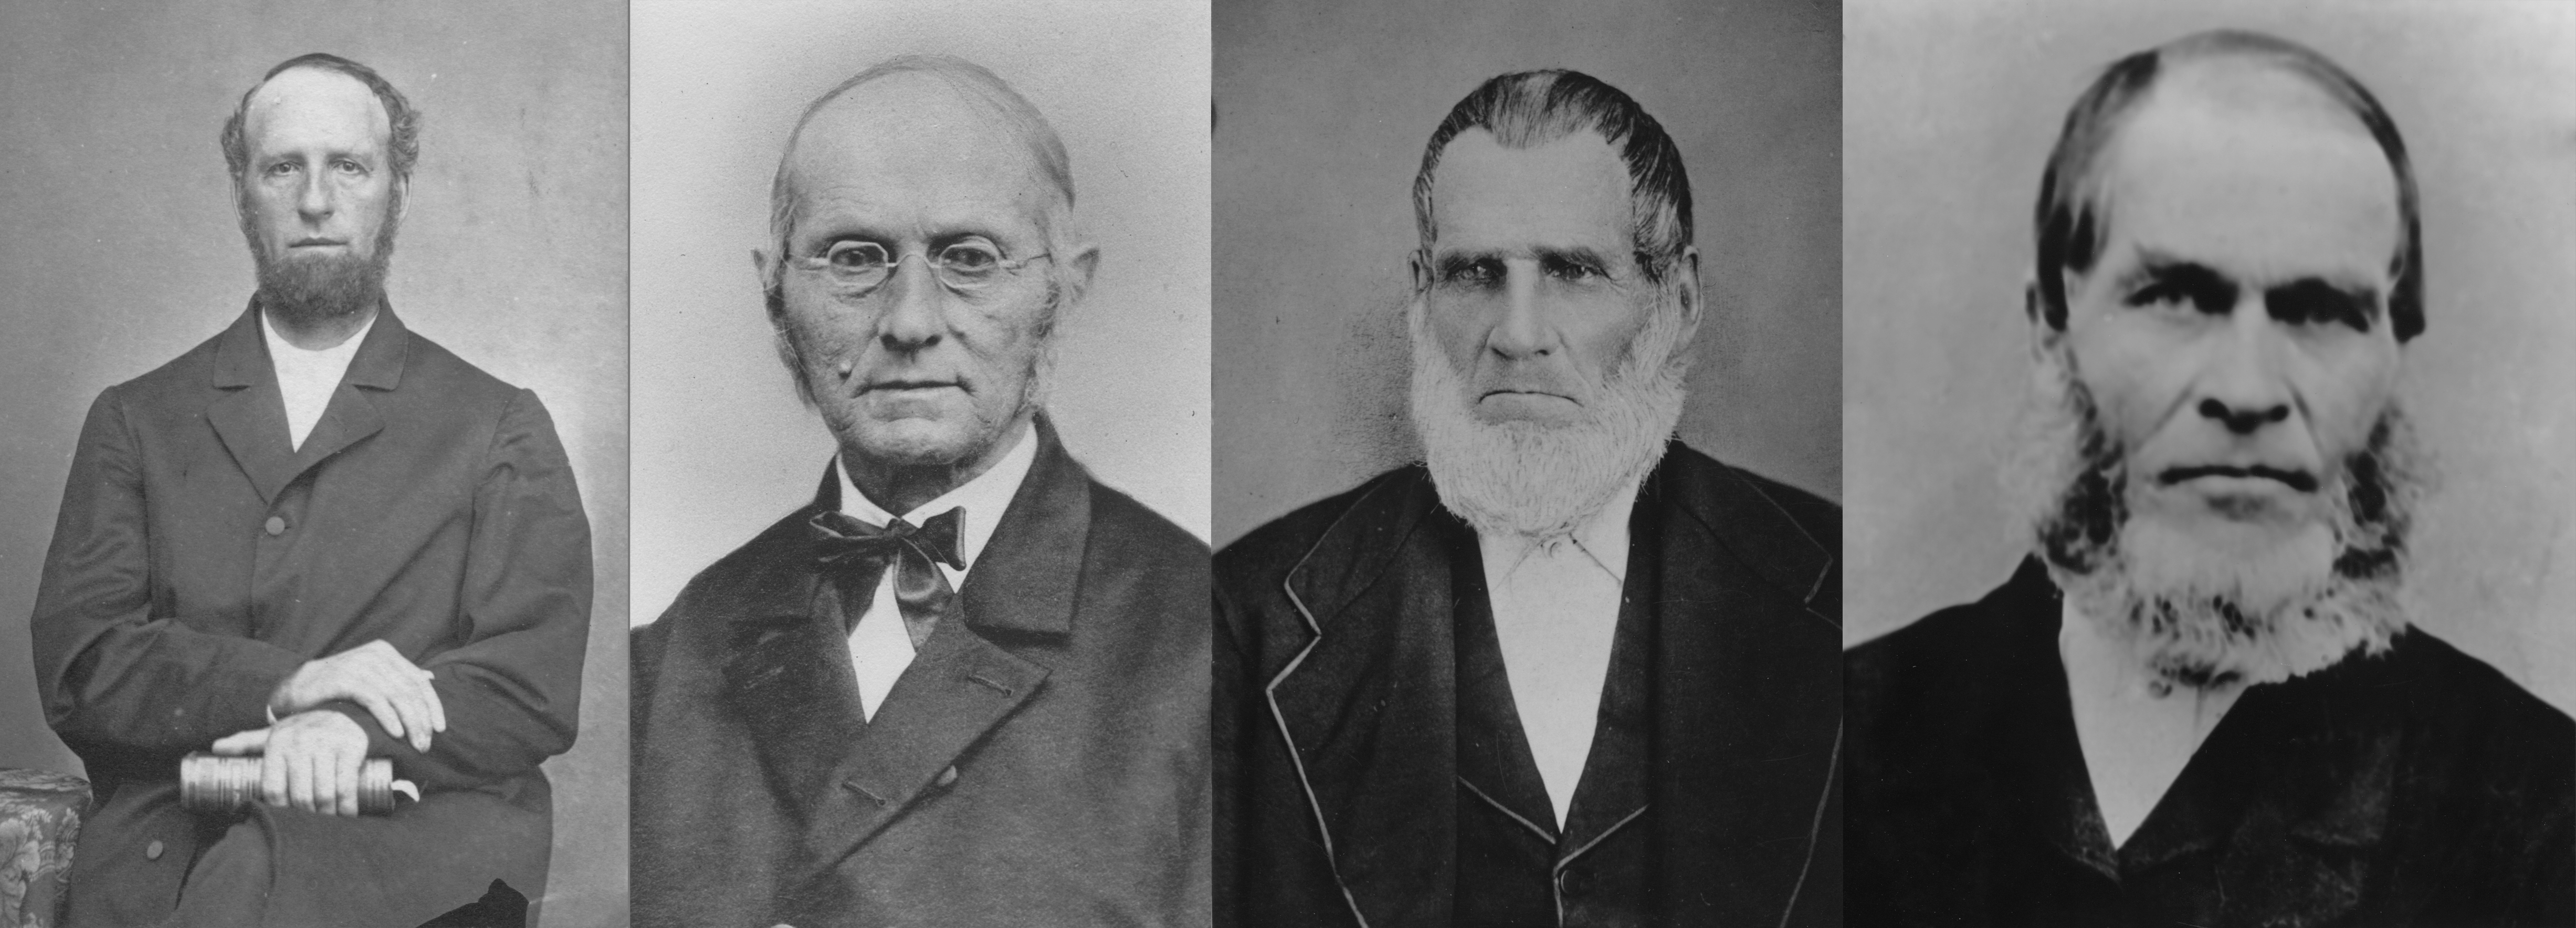
\includegraphics[width=1\linewidth]{images/james-white-joseph-bates-stephen-pierce-hiram-edson.jpg}
    \caption*{James White, Joseph Bates, Stephen Pierce, Hiram Edson}
    \label{fig:pioneers}
\end{figure}

\egwnogap{Przez cały ten czas nie mogłam zrozumieć rozumowania braci. Mój umysł był jakby zablokowany i nie mogłam pojąć znaczenia studiowanych przez nas fragmentów Pisma Świętego. Był to jeden z największych smutków mojego życia. \textbf{Pozostawałam w tym stanie umysłu, dopóki wszystkie \underline{główne punkty naszej wiary} nie zostały wyjaśnione w naszych umysłach, w harmonii ze Słowem Bożym}. Bracia wiedzieli, że gdy nie byłam w widzeniu, nie mogłam zrozumieć tych spraw, i przyjmowali objawienia jako światło bezpośrednio z nieba}[SpTB02 57.1; 1904][https://egwwritings.org/read?panels=p417.291]

\egwnogap{Przez dwa lub trzy lata mój umysł pozostawał zamknięty na zrozumienie Pisma Świętego. W trakcie naszej pracy, mój mąż i ja odwiedziliśmy ojca Andrews, który cierpiał na silny reumatyzm zapalny. Modliliśmy się za niego. Położyłam ręce na jego głowie i powiedziałam: «Ojcze Andrews, Pan Jezus cię uzdrawia». Został uzdrowiony natychmiast. Wstał i chodził po pokoju, chwaląc Boga i mówiąc: «Nigdy wcześniej nie widziałem czegoś takiego. Aniołowie Boży są w tym pokoju». Chwała Pańska została objawiona. Światło zdawało się świecić w całym domu, a ręka anioła została położona na mojej głowie. Od tamtego czasu aż do teraz jestem w stanie rozumieć Słowo Boże}[SpTB02 57.2; 1904][https://egwwritings.org/read?panels=p417.292]

\egwnogap{\textbf{Jaki wpływ skłania ludzi na tym etapie naszej historii do działania w ukryty, potężny sposób, aby \underline{zburzyć fundament naszej wiary} — fundament, który został położony na początku naszej pracy poprzez pełne modlitwy studium Słowa i przez objawienie? Na \underline{tym fundamencie} budujemy przez \underline{ostatnie pięćdziesiąt lat}. Czy dziwicie się, że gdy widzę początek działalności, która \underline{dąży do usunięcia niektórych z filarów naszej wiary}, mam coś do powiedzenia? Muszę być posłuszna rozkazowi: «Staranuj ją!»}}[SpTB02 58.1; 1904][https://egwwritings.org/read?panels=p417.295]

\egwnogap{Żywię najczulsze uczucia wobec dr. Kellogga. Przez wiele lat starałam się za nim obstawać. Słowo Boże zawsze mówiło mi: «Możesz mu pomóc». Czasami budzę się w nocy i chodząc po pokoju, modlę się: «O Panie, trzymaj dr. Kellogga mocno. Nie pozwól mu odejść. Zachowaj go niezłomnym. Namaść jego oczy niebiańską maścią, aby mógł widzieć wszystko wyraźnie». Noc po nocy leżałam bezsennie, zastanawiając się, jak mogę mu pomóc. Gorliwie i często modliłam się, aby Pan nie pozwolił mu odwrócić się od uświęcającej prawdy. To jest ciężar, który mnie przygniata — pragnienie, aby nie popełniał błędów, które zraniłyby jego duszę i \textbf{zaszkodziły sprawie teraźniejszej prawdy}. Ale od pewnego czasu jego działania ujawniają, że kieruje nim dziwny duch. Pan weźmie tę sprawę w swoje ręce. Muszę nieść poselstwa ostrzeżenia, które Bóg mi daje, a następnie pozostawić Panu rezultaty. \textbf{Muszę teraz przedstawić tę sprawę we wszystkich jej aspektach, ponieważ lud Boży nie może zostać splądrowany}}[SpTB02 58.2; 1904][https://egwwritings.org/read?panels=p417.296]

\egwnogap{\textbf{Jesteśmy zachowującym przykazania ludem Bożym. Przez ostatnie pięćdziesiąt lat była kierowana przeciwko nam każda forma herezji, aby zaciemnić nasze umysły w odniesieniu do nauczania Słowa} — \textbf{szczególnie odnośnie do służby Chrystusa w niebiańskiej świątyni i poselstwa niebios na te ostatnie dni, danego przez aniołów z czternastego rozdziału Księgi Objawienia}. \textbf{Poselstwa wszelkiego rodzaju i typu były narzucane Adwentystom Dnia Siódmego, aby zastąpić prawdę, która \underline{punkt po punkcie} została odkryta przez pełne modlitwy studium i potwierdzona przez cudotwórczą moc Pana}. \textbf{Lecz \underline{drogowskazy}, które \underline{uczyniły nas tym, czym jesteśmy}, \underline{mają być zachowane} i \underline{będą zachowane}, jak Bóg oznajmił przez swoje słowo i świadectwo swojego Ducha}. \textbf{Wzywa nas, abyśmy \underline{trzymali się mocno}, z uściskiem wiary, \underline{fundamentalnych zasad}, które są \underline{oparte na niepodważalnym autorytecie}}}[SpTB02 59.1; 1904][https://egwwritings.org/read?panels=p417.299]

Istniała konieczność ostrzeżenia Kościoła przed działaniem wroga zmierzającym do wykorzenienia fundamentu naszej wiary. Istniała konieczność przypomnienia Kościołowi, co stanowi prawdziwy fundament wiary Adwentystów Dnia Siódmego. Wydaje się, że Adwentyści Dnia Siódmego w tamtym czasie zapominali drogi, którą  \egwinline{Pan nas prowadził, oraz Jego nauk w naszej dotychczasowej historii.}[LS 196.2; 1915][https://egwwritings.org/read?panels=p41.1083]

\egw{Jaki wpływ skłania ludzi na tym etapie naszej historii do działania w ukryty, potężny sposób, aby \textbf{zburzyć fundament naszej wiary} - fundament, który został położony \textbf{na początku naszego dzieła} poprzez pełne modlitwy studium Słowa i przez objawienie? Na \textbf{tym fundamencie} budujemy przez \textbf{ostatnie pięćdziesiąt lat}. Czy dziwicie się, że gdy widzę początek działalności, która \textbf{dąży do usunięcia niektórych z filarów naszej wiary}, mam coś do powiedzenia? Muszę być posłuszna rozkazowi: «\textbf{Przeciwstaw się temu}!»}[SpTB02 58.1; 1904][https://egwwritings.org/read?panels=p417.295]

Czemu siostra White zgodnie z tym poleceniem miała się przeciwstawić?

\egwinline{Mniej więcej w czasie, gdy opublikowano «The Living Temple»}, w porze nocnej zobaczyła ona \egwinline{obrazy wskazujące, że zbliża się jakieś niebezpieczeństwo}, i że musi się na nie \egwinline{przygotować poprzez spisanie rzeczy, które Bóg jej objawił} \egwinline{\textbf{odnośnie do fundamentalnych zasad naszej wiary}.}

Została \egwinline{pouczona przez niebiańskiego posłańca, że część rozumowania w książce «The Living Temple» jest niepoprawna i że \textbf{to rozumowanie sprowadziłoby na manowce} umysły tych, którzy nie są całkowicie utwierdzeni w \textbf{fundamentalnych zasadach} teraźniejszej prawdy.}

Więc jaki był faktyczny problem z książką «The Living Temple»?

Jeśli jesteś uczonym, historykiem adwentystycznym, teologiem lub po prostu studentem teologii, zanim udzielisz prostej odpowiedzi i powiesz, że problemem był panteizm, chcielibyśmy zwrócić Twoją uwagę z powrotem na tekst. Siostra White jasno określiła istotę problemu, stwierdzając, że «The Living Temple» \egwinline{wprowadza to, co jest niczym innym jak spekulacją w \textbf{odniesieniu do osobowości Boga i tego, gdzie jest Jego obecność}.}

Nie zaprzeczamy panteistycznemu problemowi książki, ale chcemy przekierować uwagę z błędu Kellogga na światło, które dał Bóg. Istnieją dwa sposoby podejścia do kryzysu Kellogga. Jeden polega na zajęciu się panteizmem, a drugi na zajęciu się \egwinline{\textbf{osobowością Boga} i \textbf{tym, gdzie jest Jego obecność}}. Jeden sposób to badanie błędu, a drugi to badanie Prawdy. Jeden sposób to analizowanie ciemności, a drugi to picie ze źródła Prawdy. Wybieramy to drugie i z tego powodu ta książka różni się od setek innych książek napisanych o kryzysie Kellogga. Tematem tej książki nie jest panteizm ani żaden inny błąd, ale prawda i to, co Bóg objawił o swojej osobowości i tym, gdzie jest Jego obecność. To był prawdziwy problem publikacji Kellogga.

Wierzymy, że studiowanie i analizowanie błędu jest bardzo niebezpieczne, ponieważ błąd prowadzi do zwiedzenia. Problem ze zwiedzeniem polega na tym, że możemy być zwiedzeni, oczywiście nie wiedząc, że jesteśmy zwiedzeni! Mocno wierzymy, że Ellen White była prorokiem Boga i że otrzymywała Światło od Boga, \bible{który jest światłością i nie ma w Nim żadnej ciemności}[1J 1:5]. Dlatego nie oczekujemy, że siostra White wyjaśni błędy w książce «The Living Temple». Wielu przychodziło do niej, prosząc ją \egwinline{o wyjaśnienie stanowisk zajętych w «The Living Temple»}. Odpowiedziała: \egwinline{Są one niewytłumaczalne}. Jej celem nie było analizowanie błędu, ale rzucenie światła Prawdy na \emcap{osobowość Boga} i to, gdzie jest Jego obecność. W ten sposób wskazywała na prawdy, na których Bóg założył Kościół Adwentystów Dnia Siódmego. Te prawdy stanowiły fundament naszej wiary. Te prawdy zostały nam dane w naszych wczesnych dniach. Przekierowując naszą uwagę z osobowości Boga na panteizm, tracimy okazję, by pamiętać \egwinline{\textbf{drogę, którą Pan nas prowadził}, i \textbf{Jego nauki} w naszej \textbf{dotychczasowej historii}}. W tym świetle wyrażamy nasze zaniepokojenie kryzysem Kellogga i jego panteistycznym podejściem, ponieważ \egwinline{ścieżka prawdy biegnie blisko ścieżki błędu i obie ścieżki mogą wydawać się być jedną}; rozwiązaniem jest bycie \egwinline{całkowicie utwierdzonym w \textbf{fundamentalnych zasadach} teraźniejszej prawdy}. W innych miejscach siostra White mocno ugruntowała tę zasadę.

\egw{Szatan wcale nie śpi; jest on w pełni rozbudzony i rozgrywa grę o życie dusz ludu Bożego. Przyjdzie do nich z wszelkiego rodzaju pochlebstwami, mając nadzieję doprowadzić ich do zboczenia z drogi wierności. \textbf{Pragnie odwrócić ich uwagę od prawdziwych kwestii ku fałszywym teoriom}.}[Ms132-1903.42; 1904][https://egwwritings.org/read?panels=p9056.56]

Skupmy więc naszą uwagę na prawdziwym problemie, a nie na fałszywych teoriach.

% Fundament naszej wiary

\begin{titledpoem}
    \stanza{
        Prawda wieczna mocno stoi, \\
        Żaden wróg jej nie rozbroi. \\
        Pan swą siłą dzieło tchnie, \\
        Wiernych posłów wspiera swe.
    }

    \stanza{
        Na platformie prawdy trwajmy, \\
        Filarów wiary się trzymajmy. \\
        To fundament dany nam, \\
        Który przetrwa czasu plan.
    }

    \stanza{
        Wróg chce usunąć prawdy te, \\
        Fałszywe teorie szerząc swe. \\
        Lecz Bóg wzbudzi wiernych swych, \\
        By strzec zasad odwiecznych tych.
    }

    \stanza{
        O Bożej osobowości nie spekulujmy, \\
        Mistycyzmu się wystrzegajmy. \\
        Ścieżka prawdy blisko błędu biegnie, \\
        Tylko Duch Święty nas bezpiecznie wiedzie.
    }
\end{titledpoem}

% Staranuj górę lodową

\begin{titledpoem}
    \stanza{
        "Staranuj ją!" - rozkaz brzmi, \\
        Gdy góra lodowa przed nami tkwi. \\
        Bez wahania naprzód płyń, \\
        By rozbić zwodniczy cień.
    }

    \stanza{
        Fundament wiary solidny jest, \\
        Przez pięćdziesiąt lat przetrwał test. \\
        Przez studiowanie i modlitwy żar, \\
        Bóg dał nam prawdy wiecznej dar.
    }

    \stanza{
        Zasady, które Bóg nam dał, \\
        By każdy wiernie przy nich stał. \\
        Nie pozwól, by je zabrał wróg, \\
        Gdy burzy to, co zbudował Bóg.
    }

    \stanza{
        Trzymajmy się więc mocno dziś, \\
        Tego, co dane nam przez Pana jest. \\
        Niech prawda jasno świeci nam, \\
        Aż wejdziemy do niebios bram.
    }
\end{titledpoem}
